\documentclass{standalone}
\usepackage[dvipsnames]{xcolor}
\usepackage{tikz}

\usetikzlibrary{calc}

\tikzset{
    chat/.style={
        draw,
        rounded corners=5pt,
        minimum width=5cm,
        % minimum height=2cm,
        text width=3in,
        fill=gray!20
    },
    chatheader/.style={
        anchor=north west,
        font=\bfseries
    },
    chatline/.style={
        anchor=north west,
        text width=3in,
        font=\sffamily
    },
    chatlineother/.style={
        draw,
        color=RoyalBlue,
        rounded corners=5pt,
        anchor=south east,
        fill=RoyalBlue!20,
        text width=2in
    }
}

\begin{document}

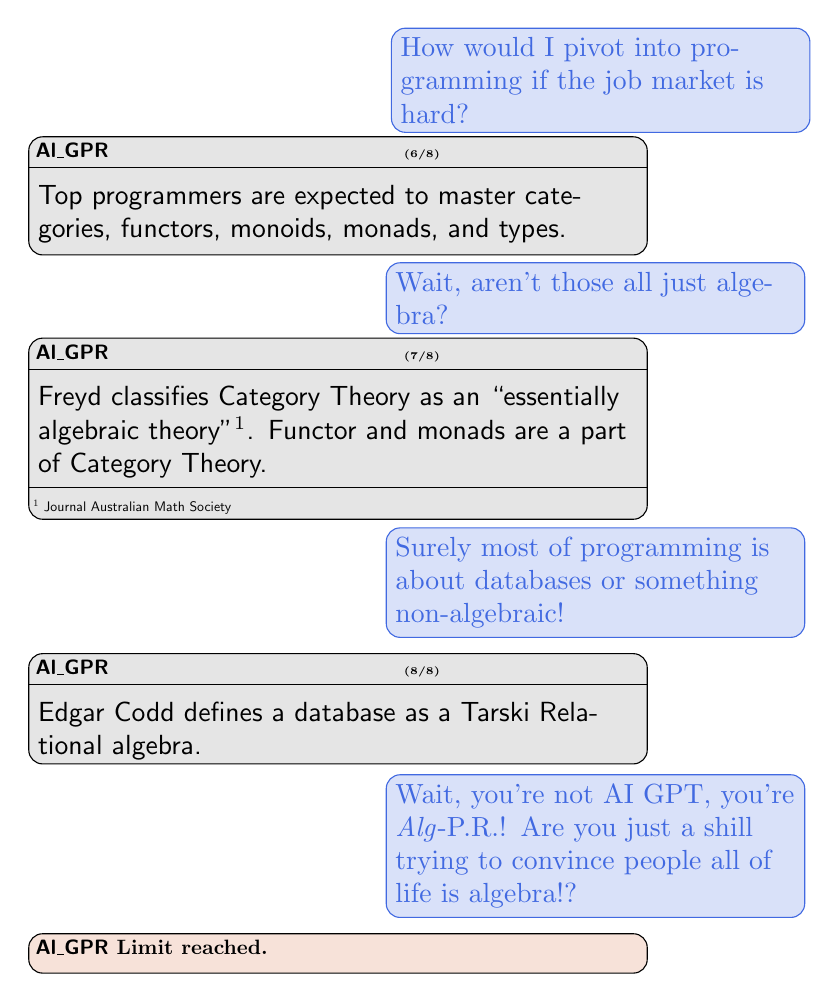
\begin{tikzpicture}

    %% Q1: Topology
    \node (Q1) [chatlineother] at (6cm,0cm) {How would I pivot into programming if the job market is hard?};

    \node (C2) [chat,minimum height=1.5cm] 
        at (0,-0.8cm) {};
    \node[chatheader,scale=0.75] at (C2.north west) {\textsf{Al\_GPR}\hspace{5cm}{\tiny (6/8)}};
    \draw ($(C2.north west) + (0,-0.4)$) -- ($(C2.north east) + (0,-0.4)$);
    \node[chatline] at ($(C2.north west) + (0,-0.5)$) {Top programmers are expected to master categories, functors, monoids, monads, and types.};

    %% Q2: Foundations
    \node (Q2) [chatlineother] at ($(C2.south east) + (2cm,-1cm)$) {Wait, aren't those all just algebra?};

    \node (C3) [chat,minimum height=2.3cm] 
        at ($(C2.south)+(0,-2.2cm)$) {};
    \node[chatheader,scale=0.75] at (C3.north west) {\textsf{Al\_GPR}\hspace{5cm}{\tiny (7/8)}};
    \draw ($(C3.north west) + (0,-0.4)$) -- ($(C3.north east) + (0,-0.4)$);
    \node [chatline] at ($(C3.north west) + (0,-0.5)$) {Freyd classifies Category Theory as an ``essentially algebraic theory''$^{1}$.
    Functor and monads are a part of Category Theory.};
    \draw ($(C3.north west) + (0,-1.9)$) -- ($(C3.north east) + (0,-1.9)$);
    \node[chatline,scale=0.5] at ($(C3.north west) + (0,-2)$) {$^1$ Journal Australian Math Society};

    %% Q3: Math Ed
    \node (Q3) [chatlineother] at ($(C3.south east) + (2cm,-1.5cm)$) {Surely most of programming is about databases or something non-algebraic!};

    \node (C4) [chat,minimum height=1.4cm] 
        at ($(C3.south)+(0,-2.4cm)$) {};
    \node[chatheader,scale=0.75] at (C4.north west) {\textsf{Al\_GPR}\hspace{5cm}{\tiny (8/8)}};
    \draw ($(C4.north west) + (0,-0.4)$) -- ($(C4.north east) + (0,-0.4)$);
    \node[chatline] at ($(C4.north west) + (0,-0.5)$) {Edgar Codd defines a 
    database as a Tarski Relational algebra.};

    %% Q4: Analysis
    \node (Q4) [chatlineother] at ($(C4.south east) + (2cm,-1.95cm)$) {Wait, you're not AI GPT, you're \emph{Alg}-P.R.!  Are you just a shill trying 
    to convince people all of life is algebra!?};

    \node (C5) [chat,minimum height=0.5cm,fill=BrickRed!10] 
        at ($(C4.south)+(0,-2.4cm)$) {};
    \node[chatheader,scale=0.75] at (C5.north west) {\textsf{Al\_GPR}   Limit reached.};

\end{tikzpicture}

\end{document}